%% =====================================================================
%%  Dumbocracy: Campaigning on a Social Network
%%  Project report (v3)
%%
%%  Build:  pdflatex main && bibtex main && pdflatex main && pdflatex main
%%          (or latexmk -pdf main, or upload this folder to Overleaf)
%% =====================================================================
\documentclass[11pt,a4paper,oneside]{report}

%% ---------- Page and fonts ------------------------------------------
\usepackage[a4paper,top=2.6cm,bottom=2.6cm,left=2.5cm,right=2.5cm,headheight=14pt]{geometry}
\usepackage[T1]{fontenc}
\usepackage[utf8]{inputenc}
\usepackage{newpxtext}            % Palatino-like text
\usepackage{newpxmath}            % matching maths
\usepackage[scaled=0.86]{beramono}% readable monospace for code names
\usepackage{microtype}
\linespread{1.08}

%% ---------- Maths, tables, figures ------------------------------------
\usepackage{mathtools}            % amsmath + extras; newpxmath already supplies the AMS symbols
\usepackage{booktabs,tabularx,array,multirow}
\usepackage{graphicx}
\usepackage[font=small,labelfont=bf,margin=0.5cm]{caption}
\usepackage{subcaption}
\usepackage{enumitem}
\setlist{itemsep=2pt,topsep=4pt,parsep=0pt}
\usepackage{xcolor}
\usepackage{tikz}
\usetikzlibrary{positioning,arrows.meta,fit,calc,shapes.geometric,backgrounds}

%% ---------- Colours ---------------------------------------------------
\definecolor{ink}{HTML}{1F2A44}
\definecolor{accent}{HTML}{2E5E8C}
\definecolor{soft}{HTML}{E8EEF5}
\definecolor{softgreen}{HTML}{E7F2EA}
\definecolor{softsand}{HTML}{F6EFE2}
\definecolor{todo}{HTML}{C0392B}

%% ---------- Headings, headers -----------------------------------------
\usepackage{titlesec}
\titleformat{\chapter}[display]
  {\normalfont\bfseries\color{ink}}
  {\large\scshape\color{accent}Chapter \thechapter}
  {4pt}
  {\Huge}
  [\vspace{2pt}{\color{accent}\titlerule[0.8pt]}]
\titlespacing*{\chapter}{0pt}{-10pt}{22pt}
\titleformat{\section}{\normalfont\Large\bfseries\color{ink}}{\thesection}{0.8em}{}
\titleformat{\subsection}{\normalfont\large\bfseries\color{ink}}{\thesubsection}{0.8em}{}
\titleformat{\subsubsection}{\normalfont\normalsize\bfseries\itshape\color{ink}}{}{0em}{}
\setcounter{secnumdepth}{2}
\setcounter{tocdepth}{1}

\usepackage{fancyhdr}
\pagestyle{fancy}
\fancyhf{}
\fancyhead[L]{\small\color{accent}\nouppercase{\leftmark}}
\fancyhead[R]{\small\color{accent}Dumbocracy}
\fancyfoot[C]{\small\thepage}
\renewcommand{\headrulewidth}{0.4pt}
\fancypagestyle{plain}{\fancyhf{}\fancyfoot[C]{\small\thepage}\renewcommand{\headrulewidth}{0pt}}

%% ---------- References and links ---------------------------------------
\usepackage[numbers,sort&compress]{natbib}
\usepackage[hidelinks]{hyperref}
\hypersetup{pdftitle={Dumbocracy: Campaigning on a Social Network},
            pdfsubject={Multi-Agent Systems course project report}}
\usepackage[nameinlink,capitalise]{cleveref}
\usepackage{url}
\urlstyle{same}

%% ---------- Macros ----------------------------------------------------
\newcommand{\todo}[1]{\textcolor{todo}{\textbf{[TODO:} #1\textbf{]}}}
\newcommand{\coins}[1]{#1~coins}
\newcommand{\simplex}{\Delta}
\newcommand{\TV}{\operatorname{TV}}
\newcommand{\E}{\mathbb{E}}
\newcommand{\R}{\mathbb{R}}
\newcommand{\code}[1]{\texttt{#1}}
\newcommand{\ORACLE}{\textsc{Oracle}}
\newcommand{\Kop}{\mathsf{K}}
\newcommand{\Mop}{\mathsf{M}}
\DeclareMathOperator*{\argmax}{arg\,max}
\DeclareMathOperator*{\argmin}{arg\,min}
\newcommand{\repo}{\url{https://github.com/saikaushhikp/CLOUT}}

%% Overview / summary sections: a light coloured rule makes them easy to find.
\newcommand{\overviewsection}{\section{Overview}}
\newcommand{\summarysection}{\section{Summary}}

%% ---------- TikZ styles -----------------------------------------------
\tikzset{
  box/.style={draw=accent,line width=0.6pt,rounded corners=3pt,fill=soft,
              align=center,inner sep=4pt,
              font=\small,
              execute at begin node={\hyphenpenalty=10000 \exhyphenpenalty=10000 }},
  sub/.style={font=\scriptsize},
  boxg/.style={box,fill=softgreen},
  boxs/.style={box,fill=softsand},
  arr/.style={-{Stealth[length=2.4mm]},line width=0.6pt,color=ink},
  darr/.style={{Stealth[length=2.4mm]}-{Stealth[length=2.4mm]},line width=0.6pt,color=ink},
}

\begin{document}

%% =====================================================================
%%  Title page
%% =====================================================================
\begin{titlepage}
\centering
\vspace*{1.2cm}
{\large\scshape\color{accent} Multi-Agent Systems \textendash{} Course Project Report\par}
\vspace{1.4cm}
{\color{ink}\rule{\linewidth}{0.8pt}\par}
\vspace{0.5cm}
{\fontsize{30}{36}\selectfont\bfseries\color{ink} Dumbocracy\par}
\vspace{0.35cm}
{\LARGE\color{ink} Campaigning on a Social Network\par}
\vspace{0.4cm}
{\large\itshape Cascades, consensus, planning under uncertainty and knowledge,\\
studied with a GPU-batched election game\par}
\vspace{0.5cm}
{\color{ink}\rule{\linewidth}{0.8pt}\par}
\vspace{1.6cm}

{\large Submitted by\par}
\vspace{0.4cm}
\begin{tabular}{ll}
\toprule
\textbf{Name} & \textbf{Roll number} \\
\midrule
\todo{Full name} (Kaushik) & AI23BTECH11017 \\
\todo{Full name} (Madhava Asrith) & \todo{roll no.} \\
\todo{Full name} (Hemanth Reddy) & \todo{roll no.} \\
\todo{Full name} (Vishank Singh) & \todo{roll no.} \\
\todo{Full name} & AI23BTECH11033 \\
\bottomrule
\end{tabular}

\vspace{1.4cm}
{\large Under the guidance of \todo{instructor name}\par}
\vspace{0.3cm}
{\large Indian Institute of Technology Hyderabad\par}
\vspace{0.3cm}
{\large November 2026\par}
\vfill
{\small Code repository: \repo\par}
\end{titlepage}

%% =====================================================================
%%  Front matter
%% =====================================================================
\pagenumbering{roman}

\chapter*{Abstract}
\addcontentsline{toc}{chapter}{Abstract}

An election campaign is a contest fought on a network. A party spends money to change what people think,
but people also change each other's minds, and the party never sees the electorate directly. We built
\emph{Dumbocracy}, a single-player election game, to study this situation with the tools of multi-agent
systems.

The electorate has between ten thousand and one million simulated voters. They live in four regions and
are linked by a friendship network. Each voter wants the government budget split across five sectors in a
particular way. The player writes a manifesto (their own budget split) and then has a few campaign rounds
to win a majority. Each round they may hire party workers, who start word-of-mouth cascades through the
network; buy regional media airings; and pay for survey questions. Meanwhile, every voter drifts towards
the average opinion of their friends.

The game connects several course topics in one place. Opinion drift is DeGroot consensus with stubborn
agents; party workers spread influence by an Independent Cascade; choosing a manifesto is an optimisation
problem on the probability simplex, which we solve with projected gradient and ADMM; and the player's
uncertainty about the electorate is described exactly by epistemic logic, with temporal logic describing
how a campaign unfolds. We implemented the whole model as one PyTorch code path that runs a single world on
a CPU or hundreds of worlds at once on a GPU, together with Bayesian and scripted computer players, a
formal-reasoning layer that tells the player after the game what they knew and when, a web interface for
human play, and an experiment harness with paired seeds and machine-checked reporting.

This report describes the model, the players, the reasoning layer and the software. The experiment suite
built on top of it is reported in \cref{ch:results}.

\tableofcontents
\clearpage
\listoffigures
\listoftables
\clearpage
\pagenumbering{arabic}

%% =====================================================================
%%  Chapter 1: Introduction
%% =====================================================================
\chapter{Introduction}\label{ch:intro}

\overviewsection

This chapter explains what problem we set out to study and why a game is a good way to study it. It
states the questions that drive the project, lists what we built, and describes how the rest of the report
is organised. It ends with a statement of who in the group did what.

\section{Motivation}

Political campaigns spend money to move opinions. Those opinions are not static: people talk to their
friends, read the news and slowly converge on what their social circle thinks. A campaign therefore pushes
on a system that is already moving by itself. Two classical families of models describe the two halves of
this picture.
\begin{itemize}
  \item \textbf{Opinion dynamics} models, such as DeGroot averaging~\cite{degroot1974}, describe how
        opinions drift towards a consensus when each person repeatedly averages the views of their
        neighbours. Stubborn agents, people whose view never changes, can stop that consensus from
        forming~\cite{friedkin1990,mobilia2003}.
  \item \textbf{Contagion} models, such as the Independent Cascade~\cite{goldenberg2001,kempe2003}, describe
        how a new idea jumps from person to person. They have a sharp threshold: below it a cascade dies
        out, above it a cascade can reach a large part of the network~\cite{chakrabarti2008}.
\end{itemize}

A real campaign also works in the dark. The party does not know exactly which regions want what, or how
easily each region can be persuaded. Every decision is made under uncertainty, and two questions keep
coming up: \emph{what do I actually know?} and \emph{can I still guarantee a win?} Epistemic logic gives
these questions precise meanings~\cite{fagin1995}, and temporal logic lets us ask when, during a campaign,
the outcome is settled~\cite{pnueli1977}.

We wanted one setting in which all of these ideas interact, rather than studying each in isolation. A game
gives exactly that. It has clear rules, a clear goal, and a player who must act with incomplete
information. Because we wrote the simulator ourselves, we can also open the box afterwards: we can replay a
game, look at the hidden electorate, and check what the player could and could not have known.

\section{The game in one paragraph}

\emph{Dumbocracy} is a single-player election game. A synthetic electorate of $N$ voters (between $10^3$
and $10^6$; $10^4$ by default) lives in four regions joined by a friendship network. Every voter has a
preferred split of a government budget over five sectors: education, welfare, agriculture, industry and
the environment. The player begins with a treasury of \coins{500} and some free public information. They
may pay for survey questions, then they commit to a manifesto: their own five-sector budget split. After
that they play five campaign rounds. In each round they may hire party workers in any region, who try to
convert their friends, and buy media airings in any region. Between rounds, voters drift towards their
friends' views. At the end there is an election, and the player wins with more than half the votes. The
regions' true preferences and personalities stay hidden throughout.

\section{Questions we asked}

The project is organised around four groups of questions.
\begin{enumerate}[label=\textbf{Q\arabic*.}]
  \item \textbf{Mechanics against theory.} Does the simulated electorate behave as course theory predicts?
        For example, does consensus speed follow the spectrum of the network, and does the worker cascade
        show the epidemic threshold that the theory of contagion predicts?
  \item \textbf{Good play.} Which strategies win? Does a player that gathers information and plans ahead
        beat simple rules of thumb, and how close do they come to the best achievable play?
  \item \textbf{Information and knowledge.} How much is a survey question worth? Can the player learn the
        hidden personalities of regions? When the game tells the player that a win was ``guaranteed'',
        how far can that statement be trusted?
  \item \textbf{Game design.} Is the game balanced, so that no fixed pattern of spending always wins? How
        much of the outcome is luck, and which design parameters matter most?
\end{enumerate}

\section{Contributions}

The project produced the following.
\begin{enumerate}
  \item \textbf{A formal model} of a campaign on a networked electorate, combining DeGroot consensus,
        stubborn agents, an Independent Cascade and a probabilistic voting rule, with a precise information
        model that separates what is public, what can be bought and what stays hidden
        (\cref{ch:model}).
  \item \textbf{Computer players} that act only on what a human could see: scripted baselines, a
        full-information reference called the \ORACLE, and a Bayesian planner that chooses survey questions
        by information gain, optimises the manifesto on the simplex, and plans spending by simulated
        rollouts (\cref{ch:players}).
  \item \textbf{A formal-reasoning layer} that evaluates epistemic statements (``a win was possible'',
        ``a win was guaranteed'') over sampled worlds consistent with the player's knowledge, and temporal
        statements over the course of a game. It drives a post-game debrief for human players
        (\cref{ch:logic}).
  \item \textbf{A GPU-first implementation}: one PyTorch code path that is bit-identical on the CPU to the
        reference simulator and runs many worlds in parallel on a GPU, together with a web interface and
        an experiment harness with paired seeds and automatic checking of every reported number
        (\cref{ch:system}).
  \item \textbf{A pre-registered experiment suite} of 23 experiments that test the game against theory
        and against its own design goals (\cref{ch:results}).
\end{enumerate}

\section{How this report is organised}

\Cref{ch:background} gives the background needed to read the rest of the report: opinion dynamics,
contagion and influence maximisation, optimisation on the simplex, planning under uncertainty, and
epistemic and temporal logic. \Cref{ch:model} defines the game precisely. \Cref{ch:players} describes the
computer players, and \cref{ch:logic} the formal-reasoning layer. \Cref{ch:system} describes the software:
the engine, GPU batching, reproducibility, the web game and the experiment harness. \Cref{ch:results}
reports the experiments. \Cref{ch:limits} discusses limitations and future work, and \cref{ch:conclusion}
concludes. The appendices list the notation, the default parameters and the commands needed to reproduce
the work. All code is public at \repo.

\section{Use of AI tools}

We used AI coding assistants while writing parts of the simulator, the tests, the experiment scripts and
the plotting code. Every design decision, every rule of the game and every experiment was decided by the
group, and all generated code was reviewed and tested before use. The text of this report was written by
the group. The group takes joint responsibility for all of its content.

\section{Who did what}\label{sec:contrib}

The table below records each member's contribution. \todo{Each member should write their own row in their
own words, as the instructions require. The areas listed are the main parts of the project, as a guide.}

\begin{table}[h]
\centering
\caption{Contribution of each group member.}
\label{tab:contrib}
\small
\begin{tabularx}{\linewidth}{@{}p{3.2cm}X@{}}
\toprule
\textbf{Member} & \textbf{Contribution} \\
\midrule
Kaushik            & \todo{e.g.\ game specification, engine, GPU batching, experiment suite, report} \\
Madhava Asrith     & \todo{describe own contribution} \\
Hemanth Reddy      & \todo{describe own contribution} \\
Vishank Singh      & \todo{describe own contribution} \\
\todo{Fifth member}& \todo{describe own contribution} \\
\bottomrule
\end{tabularx}
\end{table}

\noindent
The main parts of the project, for reference, were: the game specification and calibration; electorate
generation and the network model; social dynamics, workers, media and voting; the information model and
game engine; the computer players and manifesto optimisers; the epistemic and temporal logic layer; the
HTTP API and web interface; testing; the experiment suite and analysis; and the writing of this report.

\summarysection

Campaigns act on opinions that also move on their own, and they do so without seeing the electorate. We
built a game that captures this and used it as a research instrument. The project asks whether the
simulated electorate follows course theory, which strategies win, what information is worth, and whether
the game is well designed. The next chapter introduces the theory that the rest of the report relies on.

%% =====================================================================
%%  Chapter 2: Background
%% =====================================================================
\chapter{Background and Related Work}\label{ch:background}

\overviewsection

The game draws on several areas that are usually taught separately. This chapter introduces each one
briefly, with only the results we use later. Readers who know a topic can skip its section. We start with
how opinions spread (consensus and contagion), move on to the optimisation methods used to pick a
manifesto, and end with planning under uncertainty and the logics of knowledge and time.

\section{Networks and random graphs}

A social network is a graph $G=(V,E)$ whose nodes are people and whose edges are friendships. We write $A$
for its adjacency matrix ($A_{ij}=1$ when $i$ and $j$ are friends), $d_i$ for the degree of node $i$, and
$D$ for the diagonal matrix of degrees. The \emph{Laplacian} is $L=D-A$. Its second-smallest eigenvalue
$\lambda_2(L)$, the algebraic connectivity, measures how well connected the graph is~\cite{fiedler1973}.

The simplest random graph is the Erd\H{o}s--R\'enyi graph, in which every pair of nodes is joined
independently with the same probability~\cite{erdos1959}. Real societies are not like that: people have
more friends in their own community. The \emph{stochastic block model} captures this by splitting nodes
into blocks and letting the link probability depend on the pair of blocks~\cite{holland1983}. Our
electorate uses a stochastic block model whose blocks are the four regions.

\section{Opinion dynamics and consensus}

In the DeGroot model~\cite{degroot1974}, each person holds an opinion $x_i$ and repeatedly replaces it with
a weighted average of their neighbours' opinions,
\begin{equation}
  x(t+1) = W\,x(t), \qquad W = D^{-1}A ,
\end{equation}
where $W$ is row-stochastic. On a connected, non-bipartite graph the opinions converge to a common value.
How fast they converge is governed by the second-largest eigenvalue modulus $\mu_2$ of $W$: the
disagreement shrinks roughly like $\mu_2^{\,t}$~\cite{olfati2007,golub2010}. A graph with weak links between
communities has $\mu_2$ close to 1 and converges slowly.

Two extensions matter for us. In the Friedkin--Johnsen model~\cite{friedkin1990}, each person keeps some
attachment to their initial opinion, so the population settles at an equilibrium instead of a consensus.
\emph{Stubborn agents} or \emph{zealots}, who never change their opinion, have a similar effect: a single
zealot can pull a whole population towards their view, and zealots with opposing views prevent consensus
altogether~\cite{mobilia2003,acemoglu2011}. Bounded-confidence models~\cite{hegselmann2002} are another
well-known variant, in which people only listen to opinions close to their own; we do not use them, but
they motivate the robustness checks below.

Finally, \emph{resilient consensus} asks how normal agents can still agree when some agents misbehave. The
W-MSR algorithm~\cite{leblanc2013} has each agent discard the $F$ most extreme neighbour values before
averaging. It succeeds if the graph is sufficiently \emph{robust}, a combinatorial property that is hard to
check exactly. In our game, party workers who never change their view are, from the network's point of
view, exactly such misbehaving agents, which makes W-MSR a natural defence to test.

\section{Contagion and influence maximisation}

The \emph{Independent Cascade} model~\cite{goldenberg2001,kempe2003} describes how an idea spreads. When a
node becomes active, it gets one chance to activate each inactive neighbour $j$, and succeeds with some
probability $q_j$. Newly activated nodes then get their own chance in the next step.

Whether a cascade fizzles out or spreads widely depends on an \emph{epidemic threshold}. For contagion on a
network, the relevant quantity is the spectral radius of the adjacency matrix weighted by the transmission
probabilities~\cite{chakrabarti2008,pastor2015}. If each neighbour $j$ is converted with probability $q_j$,
the expected number of new activations in the next step grows like the operator $A\,D_q$, where
$D_q=\operatorname{diag}(q)$. The cascade grows when $\lambda_{\max}(A D_q) > 1$ and dies out otherwise.

\emph{Influence maximisation} asks which $k$ seed nodes to activate so that the expected spread is largest.
Kempe, Kleinberg and Tardos~\cite{kempe2003} showed that the expected spread under the Independent Cascade
is a \emph{submodular} function of the seed set: each new seed adds less than the previous one. For
submodular functions, the greedy algorithm is guaranteed to reach at least $1-1/e\approx 63\%$ of the
optimum~\cite{nemhauser1978}. The CELF algorithm~\cite{leskovec2007} makes greedy selection much faster by
updating marginal gains lazily. Our party workers are seeds of exactly such a cascade, so these results
tell us what to expect from hiring them.

\section{Voting on a policy space}

In the spatial theory of voting~\cite{downs1957,enelow1984}, each voter has an ideal point in a space of
policies, and votes for the candidate whose platform is closest. Our voters' ideal points are budget
splits, so the policy space is the probability simplex
\begin{equation}
  \simplex = \Bigl\{\, x \in \R^5 : x_k \ge 0,\ \textstyle\sum_{k} x_k = 1 \,\Bigr\}.
\end{equation}
We measure the distance between two budget splits by the \emph{total-variation} distance
$\TV(x,y)=\tfrac12\lVert x-y\rVert_1$, which is the share of the budget that would have to move to turn
one split into the other. Instead of a hard ``closest platform wins'' rule, we use a probabilistic vote: a
voter supports the party with a probability that rises smoothly as the manifesto gets closer to their
ideal point.

\section{Optimisation on the simplex}

Choosing a manifesto means maximising a smooth but non-concave function over $\simplex$. We use four
first-order methods.
\begin{itemize}
  \item \textbf{Projected gradient.} Take a gradient step, then project back onto $\simplex$. The
        Euclidean projection onto the simplex can be computed exactly in $O(n\log n)$
        time~\cite{duchi2008}. It is the \emph{proximal operator} of the simplex's indicator function, so
        projected gradient is a special case of the proximal gradient method~\cite{parikh2014}.
  \item \textbf{Mirror descent.} Replace the Euclidean geometry with the entropy, which gives
        multiplicative updates that stay inside the simplex automatically~\cite{beck2003}.
  \item \textbf{Frank--Wolfe.} Move towards the vertex of the simplex that best aligns with the gradient.
        No projection is needed~\cite{frank1956,jaggi2013}.
  \item \textbf{ADMM.} Split a problem into pieces that are solved separately and then forced to
        agree~\cite{boyd2011}. In \emph{consensus} form, each region keeps its own copy of the manifesto,
        and a shared variable pulls the copies together. This is the textbook model of distributed
        optimisation in a multi-agent system.
\end{itemize}
For black-box search over whole campaign plans we also use the \emph{cross-entropy method}, which
repeatedly samples candidate plans, keeps the best fraction and refits the sampling distribution to
them~\cite{rubinstein1999}.

\section{Planning under uncertainty}

A player who does not know the hidden state of the world faces a partially observable decision
problem~\cite{kaelbling1998}. Solving such problems exactly is intractable at our scale, so we use two
standard approximations. First, the player keeps a \emph{belief}: a probability distribution over the
possible hidden worlds, updated by Bayes' rule as observations arrive. Second, the player plans by
\emph{rollouts}~\cite{bertsekas1997}: for each candidate action, it simulates the rest of the game in
several worlds sampled from its belief, follows a fixed default policy afterwards, and picks the action
with the best average result.

Information has a price in our game, so the player must also decide which question to ask. Bayesian
experimental design suggests asking the question whose answer is expected to reduce uncertainty the most,
that is, the question with the largest expected information gain (mutual information between the hidden
state and the answer)~\cite{lindley1956,chaloner1995}.

\section{Epistemic and temporal logic}

\emph{Epistemic logic}~\cite{fagin1995} formalises knowledge. An agent considers a set of worlds possible
given what it has observed. It \emph{knows} a statement $\varphi$, written $\Kop\varphi$, if $\varphi$ is
true in every world it considers possible, and it considers $\varphi$ \emph{possible}, written
$\Mop\varphi$, if $\varphi$ is true in at least one of them; the two are dual, $\Mop\varphi \equiv
\lnot\Kop\lnot\varphi$. When the ``considers possible'' relation is an equivalence relation, the logic is
called S5. This fits a player who remembers everything they observed: two worlds are indistinguishable
exactly when they would have produced the same observations. A subtle but important distinction is between
\emph{knowing that} a winning plan exists (in each possible world some plan wins, but perhaps a different
one) and \emph{knowing how} to win (one plan wins in every possible world).

\emph{Temporal logic} describes how properties change over time. Linear temporal logic (LTL)~\cite{pnueli1977}
has operators such as ``eventually'' ($\Diamond$), ``always'' ($\Box$) and ``until''. Computation tree
logic, or CTL \cite{clarke1986}, quantifies over branching futures (``on some path'' and ``on all paths''),
and alternating-time temporal logic~\cite{alur2002} asks whether an agent has a strategy that forces a
property. Signal temporal logic (STL)~\cite{maler2004} adds real-valued signals, and its \emph{robustness}
semantics~\cite{donze2010} measures by how much a property is satisfied or violated, not only whether it
is. In our game, the vote margin is such a signal.

\section{Multi-agent systems and games as instruments}

The game is a multi-agent system in the sense of~\cite{wooldridge2009,shoham2009}: thousands of simple
agents (voters) follow local rules, and one strategic agent (the party) tries to steer the collective
outcome while reasoning about what it knows. Studying such systems through simulation is common, and
textbooks such as~\cite{easley2010} use small network models to explain how behaviour spreads. What is
less common is to put the full set of tools, from spectral graph theory to epistemic logic, around one
model, and to check each prediction with controlled experiments. That is the aim of this project.

\summarysection

Opinions in our game drift by DeGroot consensus, slowed by stubborn agents and by weak links between
regions. Party workers spread influence by an Independent Cascade, which has a spectral threshold and
diminishing returns. The manifesto is chosen by optimisation on the simplex, using projected gradient,
mirror descent, Frank--Wolfe or ADMM. The player plans with a Bayesian belief and rollouts, asks questions
by information gain, and its knowledge is described by S5 epistemic logic and its progress by temporal
logic. The next chapter defines the game itself.

%% =====================================================================
%%  Chapter 3: The model
%% =====================================================================
\chapter{The Game Model}\label{ch:model}

\overviewsection

This chapter defines the game precisely. We describe how an electorate is generated, how voters change
their minds, what the player can do, how the election is decided and what the player is allowed to see.
Every rule in this chapter is implemented exactly as stated in the code, and the default values are those
used in the third version (v3) of the game. \Cref{tab:params} in \cref{app:notation} collects all default
parameters in one place.

\section{The electorate}

\subsection{Regions}

The $N$ voters are split into four regions, called North, South, East and West. Every region holds at
least 15\% of the voters, and the rest are split at random. Concretely, with $m=\lceil 0.15N\rceil$,
\begin{equation}
  \pi \sim \operatorname{Dirichlet}(2,2,2,2), \qquad
  n_r = m + \bigl[\operatorname{Multinomial}(N-4m,\ \pi)\bigr]_r ,
\end{equation}
so that $\sum_r n_r = N$ and $n_r \ge m$ for every region $r$.

\subsection{The friendship network}

Friendships form a stochastic block model whose blocks are the regions. For each game we draw ten
connection probabilities: one inside each region, $p_r \sim U[0.5, 0.9]$, and one for each pair of
regions, $p_{rs} \sim U[0.01, 0.2]$. Using them directly would make the graph almost complete, so we scale
all of them by a single sparsity factor $s$ that keeps their ratios but sets the expected mean degree to
$\bar k = 30$:
\begin{equation}
  P_{rr} = s\,p_r, \qquad P_{rs} = s\,p_{rs}, \qquad
  s = \frac{\bar k\,N}{\sum_r p_r\,n_r(n_r-1) + \sum_{r\neq s} p_{rs}\,n_r n_s}.
\end{equation}
Inside each block, every pair of voters is linked independently with probability $P$. With typical draws
about three quarters of a voter's friends live in their own region. Edges are unweighted. The player is
told the number of voters in each region and the number of friendships inside and between regions, but
never the edges themselves.

\subsection{What voters want: archetypes}

Each voter $i$ holds a preferred budget split $v_i \in \simplex$ over the five sectors, in the order
education, welfare, agriculture, industry, environment. Regions differ in what they want. There is a
public library of six \emph{archetypes} (\cref{tab:archetypes}), and a hidden one-to-one map $\sigma$
assigns one archetype to each region; there are $6\cdot5\cdot4\cdot3 = 360$ such maps. A voter in region
$r$ starts at
\begin{equation}
  v_i(0) \sim \operatorname{Dirichlet}\bigl(\kappa\,\mu_{\sigma(r)}\bigr), \qquad \kappa = 60,
\end{equation}
so voters in the same region want similar but not identical things.

\begin{table}[t]
\centering
\caption{The public archetype library. Each row is the mean budget split $\mu$ of one archetype.}
\label{tab:archetypes}
\small
\begin{tabular}{@{}llccccc@{}}
\toprule
ID & Name & Education & Welfare & Agriculture & Industry & Environment \\
\midrule
A0 & Agrarian heartland & 0.15 & 0.20 & 0.40 & 0.10 & 0.15 \\
A1 & Industrial belt    & 0.15 & 0.15 & 0.10 & 0.45 & 0.15 \\
A2 & Green urban        & 0.25 & 0.10 & 0.10 & 0.15 & 0.40 \\
A3 & Welfare-reliant    & 0.15 & 0.45 & 0.15 & 0.10 & 0.15 \\
A4 & Knowledge hub      & 0.40 & 0.10 & 0.10 & 0.25 & 0.15 \\
A5 & Balanced middle    & 0.20 & 0.20 & 0.20 & 0.20 & 0.20 \\
\bottomrule
\end{tabular}
\end{table}

\subsection{How voters can be moved: personalities}

Voters also differ in how easily they are moved. Each voter has three susceptibilities in $[0,1]$: to
friends ($\alpha_i$), to media ($\beta_i$) and to canvassing by party workers ($\gamma_i$). Each region has
one of four public \emph{personalities} (\cref{tab:personalities}), assigned by a hidden permutation
$\tau$ (24 possibilities), and voters draw their susceptibilities from that personality's Beta
distributions.

\begin{table}[t]
\centering
\caption{The public personality library. Each voter draws its susceptibilities from the Beta distributions
of its region's personality.}
\label{tab:personalities}
\small
\begin{tabular}{@{}llccc@{}}
\toprule
ID & Name & Friends $\alpha$ & Media $\beta$ & Canvassing $\gamma$ \\
\midrule
P0 & Socially driven         & Beta(6,3) & Beta(2,5) & Beta(3,4) \\
P1 & Media-savvy             & Beta(3,4) & Beta(6,3) & Beta(2,5) \\
P2 & Independent             & Beta(2,6) & Beta(2,6) & Beta(2,6) \\
P3 & Receptive to canvassing & Beta(3,4) & Beta(3,4) & Beta(6,3) \\
\bottomrule
\end{tabular}
\end{table}

Finally, each voter is independently a \emph{zealot} with probability $\zeta = 0.05$. Zealots never change
their mind ($\alpha=\beta=\gamma=0$), but their friends still listen to them.

The pair $\theta = (\sigma,\tau)$ is the \emph{hidden type} of the world; there are $360 \times 24 = 8640$
of them. Everything else (the graph, the individual preferences, the susceptibilities and the zealots) is
the \emph{micro-state}. The player's main task in gathering information is to narrow down $\theta$.

\section{Voting}

Voter $i$'s agreement with a manifesto $b$ is one minus the total-variation distance,
\begin{equation}
  S_i = 1 - \tfrac12\,\lVert v_i - b \rVert_1 \in [0,1].
\end{equation}
On election day the voter supports the party with probability
\begin{equation}\label{eq:vote}
  P_i = \frac{1}{1+\exp\bigl(-\beta_v\,(S_i - z)\bigr)}, \qquad \beta_v = 20,\quad z = 0.825 .
\end{equation}
A voter whose agreement equals the threshold $z$ votes for the party half the time; the slope $\beta_v$
controls how sharply support rises around it. We call
\begin{equation}
  E = \frac{1}{N}\sum_{i=1}^{N} P_i
\end{equation}
the \emph{expected vote share}. It is the main quantity the player tries to raise, and the one we analyse.
The official result is a seeded random draw in which each voter votes independently with probability
$P_i$. The party wins if it receives more than $N/2$ votes; a tie is a loss.

\section{What the player can do}

\subsection{Turn structure}

A game has three phases (\cref{fig:flow}). In the \emph{survey} phase the player may buy survey questions
and then commits a manifesto $b \in \simplex$, which is fixed for the rest of the game. In each of the $T$
\emph{campaign rounds} ($T=5$ by default; the web game allows 3 to 5) the player chooses an allocation: how
many workers to hire in each region and which regions to air media in. They may also ask further survey
questions. After the last round the \emph{election} is held. The treasury starts at \coins{500} (the player
may choose up to \coins{1000}), and unspent money is worth nothing.

\begin{figure}[t]
\centering
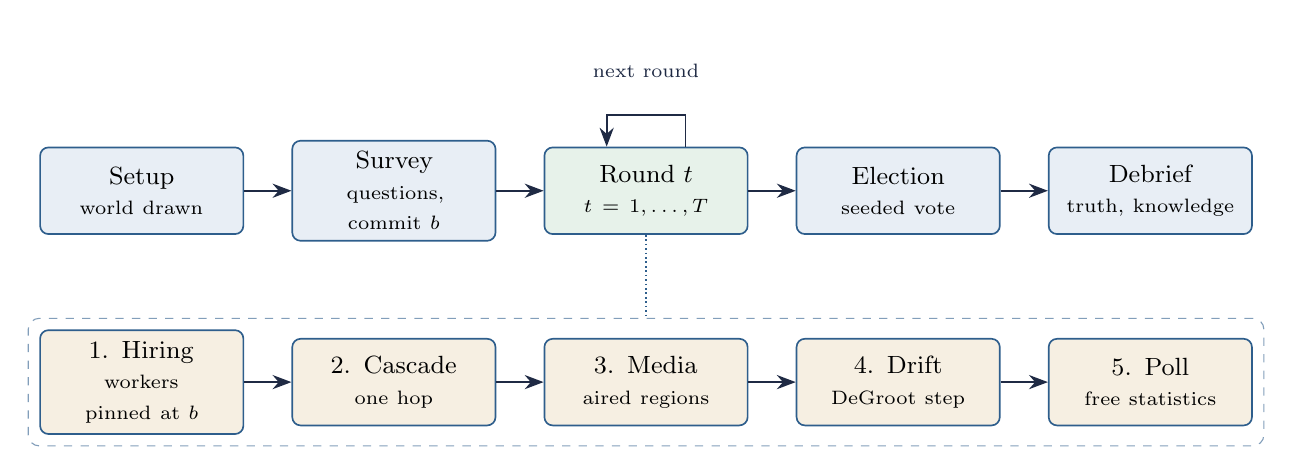
\begin{tikzpicture}[node distance=5mm and 6mm,
    every node/.append style={minimum height=11mm}]
  % top row: phases
  \node[box,text width=2.3cm] (setup) {Setup\\{\scriptsize world drawn}};
  \node[box,text width=2.3cm,right=of setup] (survey) {Survey\\{\scriptsize questions, commit $b$}};
  \node[boxg,text width=2.3cm,right=of survey] (round) {Round $t$\\{\scriptsize $t = 1,\dots,T$}};
  \node[box,text width=2.3cm,right=of round] (elec) {Election\\{\scriptsize seeded vote}};
  \node[box,text width=2.3cm,right=of elec] (debrief) {Debrief\\{\scriptsize truth, knowledge}};
  \draw[arr] (setup) -- (survey);
  \draw[arr] (survey) -- (round);
  \draw[arr] (round) -- (elec);
  \draw[arr] (elec) -- (debrief);
  \draw[arr] ([xshift=5mm]round.north) -- ++(0,4mm) -| node[pos=0.25,above,font=\scriptsize]{next round}
             ([xshift=-5mm]round.north);
  % bottom row: inside a round
  \node[boxs,text width=2.3cm,below=12mm of setup] (r1) {1. Hiring\\{\scriptsize workers pinned at $b$}};
  \node[boxs,text width=2.3cm,right=of r1] (r2) {2. Cascade\\{\scriptsize one hop}};
  \node[boxs,text width=2.3cm,right=of r2] (r3) {3. Media\\{\scriptsize aired regions}};
  \node[boxs,text width=2.3cm,right=of r3] (r4) {4. Drift\\{\scriptsize DeGroot step}};
  \node[boxs,text width=2.3cm,right=of r4] (r5) {5. Poll\\{\scriptsize free statistics}};
  \draw[arr] (r1) -- (r2);
  \draw[arr] (r2) -- (r3);
  \draw[arr] (r3) -- (r4);
  \draw[arr] (r4) -- (r5);
  \begin{scope}[on background layer]
    \node[draw=accent!60,dashed,rounded corners=4pt,fit=(r1)(r5),inner sep=4pt,minimum height=0pt] (inner) {};
  \end{scope}
  \draw[densely dotted,line width=0.6pt,color=accent] (round.south) -- (inner.north -| round.south);
\end{tikzpicture}
\caption{The flow of a game (top) and the order of events inside one campaign round (bottom).}
\label{fig:flow}
\end{figure}

\subsection{Party workers and the cascade}

A worker costs \coins{20}, paid once. When the player hires a worker in region $r$, the game picks a random
voter of that region who has at least three friends and is not a zealot or already a worker. That voter's
preference is set to the manifesto, $v_i = b$, and stays there for the rest of the game: friends and media
never move a worker. In the language of \cref{ch:background}, workers are stubborn agents placed by the
party.

Workers also start an Independent Cascade that advances one hop per round:
\begin{itemize}
  \item The \emph{spreaders} of round $t$ are the workers hired in round $t$ together with the voters
        converted in round $t-1$.
  \item Each spreader tries once to convert each of its friends $j$ (workers and zealots cannot be
        targeted). If $j$ receives $e_j$ attempts this round, it converts with probability
        \begin{equation}\label{eq:convert}
          1 - \bigl(1 - \gamma_j P_j\bigr)^{e_j},
        \end{equation}
        where $P_j$ is $j$'s current probability of voting for the party, from \cref{eq:vote}.
  \item A converted voter jumps to $v_j = b$ and spreads in the next round only. After that it is an
        ordinary voter again and drifts with its friends.
  \item No voter can receive more than three attempts in the whole game, failures included.
\end{itemize}
The factor $P_j$ in \cref{eq:convert} is a deliberate design choice: voters who already lean towards the
manifesto are easier to convert. It also couples the two halves of the game. A manifesto close to what a
region wants raises $P_j$ there, which raises the conversion chance and can push that region's cascade
above its epidemic threshold.

\subsection{Media}

Media airings target whole regions. Airing in region $r$ costs $m_0\, n_r / (N/4)$ with $m_0 = 50$, so a
quarter-sized region costs \coins{50}. Each voter in an aired region is reached with probability
$p_m = 0.6$, and a reached voter feels a pull towards $b$ of strength
\begin{equation}
  e_i = \eta_m(n)\,\beta_i, \qquad \eta_m(n) = \frac{\eta_0}{1+\lambda n},\quad \eta_0 = 0.25,\ \lambda = 0.5,
\end{equation}
where $n$ counts the player's earlier airings in that region. Repeated airings in the same region therefore
have diminishing returns.

\section{How opinions change}

Once the round's hiring, cascade and media are resolved, every voter updates at the same time. Let
$a_i = \omega\,\alpha_i$ with $\omega = 0.15$ be the weight voter $i$ gives to friends, and $c_i$ the
combined campaign pull on $i$ this round. The update is
\begin{equation}\label{eq:update}
  v_i \leftarrow (1 - a_i - c_i)\,v_i \;+\; a_i\,\bar v_{\mathcal N(i)} \;+\; c_i\, b,
  \qquad
  \bar v_{\mathcal N(i)} = \frac{1}{d_i}\sum_{j \in \mathcal N(i)} v_j ,
\end{equation}
where $\mathcal N(i)$ is the set of $i$'s friends. If $a_i + c_i$ would exceed 1, the campaign pull is
scaled down so that it does not. The new preference is a convex combination of points of the simplex, so it
stays in the simplex. Zealots and workers do not update. The friend term is exactly the DeGroot rule, and
with W-MSR switched on (an option we test) the most extreme friends are dropped before averaging.

\section{What the player can see}

The information model separates three kinds of facts.
\begin{description}[leftmargin=0pt,style=nextline]
  \item[Public at all times.] The rules and prices, $N$ and $T$, the size of each region, the archetype
        and personality libraries (but not $\sigma$ or $\tau$), the player's own treasury and actions, and a
        network census (friendship counts inside and between regions).
  \item[Free each round.] For every sector, the share of all voters who rank it among their top three, and
        a national poll of 400 random voters with its margin of error.
  \item[Paid, \coins{10} each.] A survey question ``in region $r$, what share of voters prefer sector $s_2$
        over sector $s_1$?'' The game answers from a fresh random sample of 10\% of the region, with a
        95\% margin of error. A question may be repeated, and repeated answers within a round are pooled.
\end{description}
The maps $\sigma$ and $\tau$, the graph, every individual preference and susceptibility, the zealots and
all seeds stay hidden. The implementation enforces this with allow-listed serialisers and tests that search
every response for hidden fields (\cref{ch:system}).

Everything the player observes is appended to a \emph{knowledge log}. A world is consistent with the log
if replaying the player's own actions in that world would have produced the same observations. This set of
consistent worlds is the player's \emph{information set}, and it is the foundation of the reasoning layer
in \cref{ch:logic}.

\section{How the rules evolved}

The rules above are the third version of the game. The first two versions taught us what did not work, and
the main changes are worth recording.
\begin{itemize}
  \item \textbf{Calibration.} Early defaults made the game either trivial or hopeless. A calibration study
        on 200 seeds tuned the voter concentration $\kappa$, the social step $\omega$, the media strength,
        and the voting slope and threshold until a uniform manifesto with no campaign rarely won and a
        well-informed campaign usually did.
  \item \textbf{Party workers.} In v2, workers were free each round and made random doorstep contacts,
        followed by a three-hop cascade within the round. In v3 there are no free workers: each worker is
        bought once, is a real voter of the network, stays pinned at the manifesto, and spreads influence
        one hop per round. This made workers a long-term investment and tied them to the network's
        structure.
  \item \textbf{Prices and choices.} The worker price was set to \coins{20} and the survey price to
        \coins{10}; the player may choose a treasury between \coins{500} and \coins{1000}; and the web
        game limits the number of rounds to between 3 and 5.
  \item \textbf{Sampled surveys.} Survey answers changed from exact regional shares to estimates from a
        10\% sample, so information is noisy and repeating a question can be worthwhile.
\end{itemize}

\summarysection

An electorate is four regions of voters linked by a stochastic block model. Each region has a hidden
archetype (what it wants) and a hidden personality (how it can be moved), and 5\% of voters are zealots.
The player commits a manifesto, then spends money over several rounds on workers, who are stubborn agents
that start a one-hop-per-round Independent Cascade, and on regional media. Voters drift towards their
friends by DeGroot averaging and vote with a probability that depends on their agreement with the
manifesto. The player sees region sizes, free statistics, polls and paid noisy surveys, but never the
hidden world. The next chapter describes the computer players that play this game.

%% =====================================================================
%%  Chapter 4: Players
%% =====================================================================
\chapter{Players and Decision Making}\label{ch:players}

\overviewsection

A human can play the game through the web interface, but to study it we need players that can play
thousands of games without supervision. This chapter describes the computer players we built. All but one
follow the same rule as a human: they see only the player's observation, never the hidden state. We first
describe the full-information \ORACLE, which breaks that rule on purpose and serves as a reference. We then
describe the Bayesian planner, our strongest observation-only player, and the methods it uses to ask
questions, choose a manifesto and plan its spending. We end with the simpler scripted players and a plan
search used to estimate how well one can do.

\section{The player interface}

Every player implements one method, \code{act(observation) -> action}. The observation is the same
allow-listed JSON object that the web interface receives, and the action is one of four kinds: ask a
survey question, commit a manifesto, allocate money for a round, or skip a round. The game engine validates
every action; a rejected action changes nothing and costs nothing. Because computer and human players use
the same interface, any computer player could, in principle, play through the web API.

\section{The full-information reference: \ORACLE}

The \ORACLE{} is told the true preferences and susceptibilities of every voter. It is not meant to be a
fair opponent but a labelled baseline, and its results are never mixed with those of observation-only
players.

\paragraph{Manifesto.} An important lesson from calibration was that the electorate on election day is
not the electorate at the start. Even without any campaign, five rounds of social averaging pull each
region towards its mean. The \ORACLE{} therefore simulates five rounds of social-only dynamics on the true
electorate, which we call the \emph{anticipated} electorate, and optimises the manifesto against that
(\cref{sec:manifesto-opt}).

\paragraph{Spending.} Each round, the \ORACLE{} estimates the marginal gain in expected vote share per coin
for each possible purchase, using the true state. For media, this is the expected change in $P_i$ over
voters who would be reached. For a worker in region $r$, it estimates the reach of a cascade with
per-attempt chance $a_r = \E_r[\gamma P]$ and mean degree $\bar k_r$ over the $L$ remaining hops,
\begin{equation}
  \text{reach}_r \approx \min\Bigl(\bar k_r a_r \sum_{h=0}^{L-1} (\bar k_r a_r)^h,\ \tfrac12 n_r\Bigr),
\end{equation}
times the expected gain per converted voter. It then buys greedily by value per coin. This is a sensible
heuristic, but it is a heuristic: nothing guarantees that it is optimal, and we test that directly in the
experiments.

\section{The Bayesian planner}

The Bayesian planner (``player II'' in the experiments) is our main observation-only player.
\Cref{fig:bayes} shows its loop. It keeps a belief about the hidden world, asks the most informative
survey questions, picks a manifesto that does well across plausible worlds, and plans each round by
simulating the future in worlds drawn from its belief.

\begin{figure}[t]
\centering
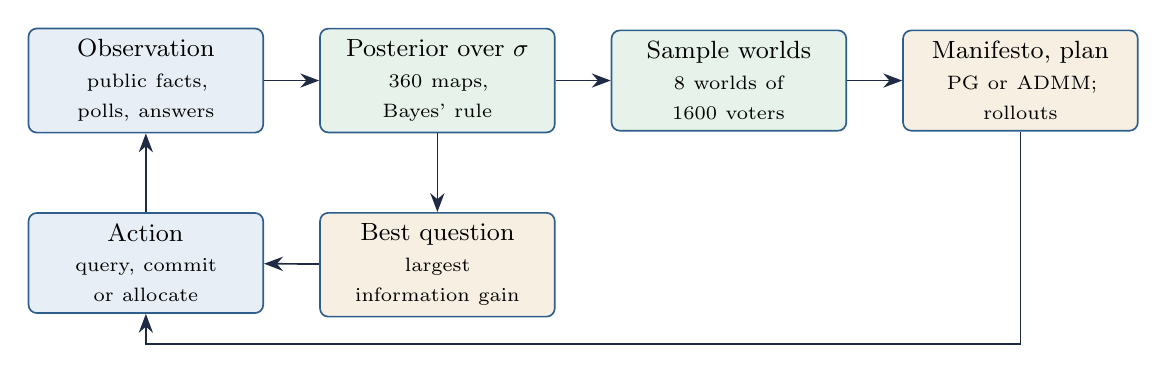
\begin{tikzpicture}[node distance=10mm and 7mm,
    every node/.append style={minimum height=12mm}]
  \node[box,text width=2.7cm] (obs) {Observation\\{\scriptsize public facts, polls, answers}};
  \node[boxg,text width=2.7cm,right=of obs] (post) {Posterior over $\sigma$\\{\scriptsize 360 maps, Bayes' rule}};
  \node[boxg,text width=2.7cm,right=of post] (worlds) {Sample worlds\\{\scriptsize 8 worlds of 1600 voters}};
  \node[boxs,text width=2.7cm,right=of worlds] (plan) {Manifesto, plan\\{\scriptsize PG or ADMM; rollouts}};
  \node[box,text width=2.7cm,below=of obs] (act) {Action\\{\scriptsize query, commit or allocate}};
  \node[boxs,text width=2.7cm,below=of post] (query) {Best question\\{\scriptsize largest information gain}};
  \draw[arr] (obs) -- (post);
  \draw[arr] (post) -- (worlds);
  \draw[arr] (worlds) -- (plan);
  \draw[arr] (post) -- (query);
  \draw[arr] (query) -- (act);
  \draw[arr] (plan.south) -- ++(0,-27mm) -| (act.south);
  \draw[arr] (act) -- (obs);
\end{tikzpicture}
\caption{One decision of the Bayesian planner. While a question is worth its price it asks one; otherwise it
commits a manifesto (in the survey phase) or chooses a round allocation (in a campaign round).}
\label{fig:bayes}
\end{figure}

\subsection{Belief over the hidden world}

Survey answers and the free top-three statistic depend only on voters' preferences, and initial
preferences depend only on the archetype map $\sigma$, not on the personalities $\tau$. The planner
therefore keeps an exact posterior over all 360 maps $\sigma$, starting from a uniform prior, and leaves
its belief over $\tau$ uniform. For each archetype, the distribution of answers to every possible question
is precomputed once by Monte Carlo. When an answer $\hat a$ arrives, every map $\sigma$ is reweighted by a
Gaussian likelihood
\begin{equation}
  \Pr(\sigma \mid \hat a) \;\propto\; \Pr(\sigma)\, \exp\!\Bigl(-\frac{(\hat a - a_\sigma)^2}{2 s^2_\sigma}\Bigr),
\end{equation}
where $a_\sigma$ is the answer expected under $\sigma$ and $s_\sigma$ combines the sampling error of a 10\%
sample with the spread of answers across voters.

\subsection{Which question to ask}

A question is a triple $(s_1, s_2, r)$: two sectors and a region. For each of the $10 \times 4 = 40$
possible questions, the planner computes the expected information gain, the mutual information between the
answer $Y$ and the archetype map,
\begin{equation}
  I(\sigma; Y) = H(\sigma) - \E_{Y}\bigl[ H(\sigma \mid Y) \bigr],
\end{equation}
and asks the question with the largest gain. It stops asking when its uncertainty is small (posterior
entropy below 0.05 nats), when the best question gains too little per coin, or after ten questions or
\coins{50} of surveys. During the campaign it may ask one more question per round if the gain is large.
Repeating a question is allowed, because each answer is a fresh sample.

\subsection{Choosing the manifesto}\label{sec:manifesto-opt}

The manifesto should maximise the expected vote share on election day,
\begin{equation}\label{eq:manifesto}
  \max_{b \in \simplex}\ f(b) = \frac{1}{N}\sum_{i} \sigma_{\mathrm{s}}\!\Bigl(\beta_v\bigl(1 - \tfrac12\lVert v_i - b\rVert_1 - z\bigr)\Bigr),
\end{equation}
where $\sigma_{\mathrm s}$ is the logistic function and $v_i$ are the voters of the anticipated electorate.
The planner does not know the $v_i$, so it builds eight synthetic worlds from its posterior: each takes a
map $\sigma$ sampled from the belief and draws everything else from the public prior, at a reduced size of
1600 voters that keeps region proportions and degree structure. It then optimises $f$ averaged over these
worlds.

The objective is not smooth, because of the absolute values, and not concave. We replace $|x|$ by the
pseudo-Huber function $\sqrt{x^2+\delta^2}-\delta$ with a small $\delta$, and run projected gradient ascent
from several starts (uniform, the population mean and the five vertices pulled towards the centre):
\begin{equation}
  b^{(k+1)} = P_{\simplex}\bigl(b^{(k)} + \eta\,\nabla \tilde f(b^{(k)})\bigr),
\end{equation}
where $P_{\simplex}$ is the exact Euclidean projection onto the simplex~\cite{duchi2008}. The best start is
chosen on the exact, unsmoothed objective.

\paragraph{The ADMM variant.} We also solve the same problem in a distributed way, as if each region
negotiated its own preferred manifesto. Writing the objective as a sum over regions,
$-f(b) = \sum_r f_r(b)$ with $f_r$ region $r$'s weighted share, consensus ADMM~\cite{boyd2011} gives each
region its own copy $x_r$ and a shared variable $z$:
\begin{align}
  x_r &\leftarrow \argmin_{x}\ f_r(x) + \tfrac{\rho}{2}\,\lVert x - z + u_r \rVert^2, \\
  z   &\leftarrow P_{\simplex}\Bigl(\tfrac14 \textstyle\sum_r (x_r + u_r)\Bigr), \\
  u_r &\leftarrow u_r + x_r - z .
\end{align}
The first step is each region's local problem, solved inexactly with a few gradient steps; the second is the
projection that enforces agreement; the third accumulates each region's disagreement. Because $f_r$ is not
convex, ADMM converges to a stationary point and needs a fairly large penalty ($\rho = 5$) and a smoother
surrogate ($\delta = 0.02$) to avoid oscillation. A third family of optimisers, mirror descent and
Frank--Wolfe, is used only in the experiments that compare optimisers.

\subsection{Planning each round}

Each round the planner builds a short list of at most twenty candidate allocations from public
information. The list always includes doing nothing, workers only, media only and mixtures, all affordable
and valid. Each candidate is scored by a rollout~\cite{bertsekas1997}: in each of the eight sampled worlds,
first replay the player's own past actions, then play the candidate this round, then follow a fixed
``even'' continuation for the remaining rounds (each round spends an equal share of the remaining money,
half on media in the least-aired regions and half on workers split by region size). The score is the mean
expected vote share on election day over the worlds, and the planner plays the best candidate. All
candidates are simulated together in one batched call using common random numbers, so differences between
candidates are not drowned out by noise.

\section{Scripted players}

To place the Bayesian planner in context we also built simpler players.
\begin{itemize}
  \item \textbf{People Pleaser (player I).} Uses the same surveys and posterior as the Bayesian planner,
        but then follows a rule of thumb. It picks the smallest group of the largest regions that together
        hold a majority, and blends the most likely archetypes of those regions, weighted by region size.
        It spends at an even pace, with media in its coalition regions and the rest on workers.
  \item \textbf{Strong-Arm (player III).} Asks no questions and pushes a fixed agenda, ignoring what voters
        want. It spends half on media in the largest regions and half on workers, at one and a half times
        the even pace, so its money runs out early.
  \item \textbf{Fixed patterns.} Simple spending rules played with a given manifesto: \emph{none} (spend
        nothing), \emph{all workers}, \emph{all media}, and \emph{split} (half and half at an even pace).
        They are used to check balance: in a well-designed game, no fixed pattern should win almost
        always.
  \item \textbf{Top-three and uniform.} Two players that ask nothing: one uses the free top-three statistic
        as its manifesto and spends evenly, and the other commits the uniform budget and never spends.
\end{itemize}

An interface for a language-model player also exists: it would receive the same observation as JSON and
reply with one action. It is not implemented, because it was outside the scope of this version.

\section{An estimate of good play: plan search}

To know how good a player is we need a target. The \ORACLE{} is one, but it is a heuristic, so we also
built an open-loop plan search. Given a manifesto and the true world, it searches over whole five-round
plans (how many workers and which media in each region, in each round). It uses the cross-entropy
method~\cite{rubinstein1999} with 256 plans per iteration, the top 10\% as the elite set, 30 iterations and
smoothing 0.7, followed by hill climbing. The final plan is re-evaluated on 20 fresh random streams so that
its score is not inflated by the noise it was selected on. This search is still a heuristic, so its score
is a lower bound on the best achievable, not the optimum itself.

\summarysection

All players except the \ORACLE{} see only what a human sees. The \ORACLE{} knows everything, optimises the
manifesto against the anticipated electorate and buys greedily by estimated value per coin. The Bayesian
planner keeps an exact posterior over the 360 archetype maps, asks the question with the largest expected
information gain, optimises the manifesto by projected gradient (or consensus ADMM) on worlds sampled from
its belief, and chooses each round's spending by batched rollouts. Scripted players and fixed patterns give
simpler points of comparison, and a cross-entropy plan search estimates how well one can do. The next
chapter describes how we reason about what each player knew.

%% =====================================================================
%%  Chapter 5: Logic
%% =====================================================================
\chapter{Reasoning About Knowledge and Time}\label{ch:logic}

\overviewsection

After a game, a player wants to know more than whether they won. Was the election already lost when they
committed the manifesto? Could they have known how to win? This chapter describes the reasoning layer that
answers such questions. We first show how we represent what the player knew at each point in the game as a
finite sample of possible worlds. We then define the epistemic properties we evaluate on that sample, and
the temporal properties we evaluate over the course of a game. Finally, we describe the debrief that
presents these results to a human player.

\section{Possible worlds}

A world $w$ consists of a hidden type $\theta=(\sigma,\tau)$ and a micro-state. Two worlds are
indistinguishable for the player, $w \sim w'$, if replaying the player's own actions in both produces the
same knowledge log. This relation is an equivalence, so the player's knowledge follows the S5 logic of
\cref{ch:background}, and the set of worlds the player considers possible at time $t$ is its information
set $I_t$, which always contains the true world.

The micro-state is continuous, so $I_t$ cannot be enumerated. Instead we draw a finite sample
$W_t \subseteq I_t$ by rejection:
\begin{enumerate}
  \item draw $\sigma$ from the Bayesian posterior over the 360 archetype maps given all statistics and
        survey answers so far;
  \item draw $\tau$ and the micro-state from the public prior, and replay the player's actions;
  \item keep the world only if its polls agree with the polls the player saw, that is, for every round,
        \begin{equation}
          \lvert \hat p_w - \hat p_{\mathrm{obs}} \rvert \;\le\; z_{\mathrm{poll}}\,
          \bigl(\mathrm{SE}(\hat p_{\mathrm{obs}}) + \epsilon\bigr), \qquad z_{\mathrm{poll}} = 2.5,\ \epsilon = 0.01 .
        \end{equation}
\end{enumerate}
Because worlds are rescaled to a smaller number of voters for speed, every statement in this chapter is a
statement about the sampled worlds, and we always report the sample size with it.

\section{Epistemic properties}

At decision point $t$, let $\Pi_t$ be a finite set of plans for the remaining rounds: ``spend nothing'' and
one plan for each candidate allocation, repeated for every remaining round. Playing every plan in every
sampled world gives an outcome matrix $V[w,\pi]$, the expected vote share on election day. A plan wins in a
world when $V[w,\pi] > 0.5$. We evaluate four properties.
\begin{align}
  \textsc{PossibleVictory}   &:\quad \exists \pi \in \Pi_t\ \exists w \in W_t:\ V[w,\pi] > 0.5, \\
  \textsc{KnowsWinExists}    &:\quad \forall w \in W_t\ \exists \pi \in \Pi_t:\ V[w,\pi] > 0.5, \\
  \textsc{GuaranteedVictory} &:\quad \exists \pi \in \Pi_t\ \forall w \in W_t:\ V[w,\pi] > 0.5, \\
  \textsc{InevitableDefeat}  &:\quad \forall \pi \in \Pi_t\ \forall w \in W_t:\ V[w,\pi] \le 0.5 .
\end{align}
The difference between the second and third lines is the difference between \emph{knowing that} a win
exists and \emph{knowing how} to win. In the second, the winning plan may differ from world to world, so
the player cannot act on it without learning more. In the third, a single plan wins everywhere the player
considers possible. Alongside these yes-or-no verdicts we report a graded confidence: the fraction of
sampled worlds in which the best plan wins.

To keep knowledge and truth separate, every epistemic field is computed only from the reconstructed
observation. A single ground-truth field, whether some plan in $\Pi_t$ would have won in the true world,
is computed separately by replaying the recorded actions through the real engine. It is shown to the
player afterwards and is never used by a player during the game.

\section{Temporal properties}

A game produces a short trace, one state per round. Each state carries Boolean atoms and one real signal:
\begin{itemize}
  \item \textsc{Lead}: the round's poll estimate is above one half;
  \item \textsc{BudgetLeft}: the treasury is not empty;
  \item \textsc{Viable} and \textsc{Guaranteed}: \textsc{PossibleVictory} and \textsc{GuaranteedVictory} at
        that round;
  \item \textsc{Victory}: the official result (true only in the final state of a won game);
  \item the margin, the poll estimate minus one half (the official share in the final state).
\end{itemize}
On these traces we evaluate bounded LTL formulas with the operators next ($X$), eventually within $k$
steps ($\Diamond_{\le k}$), always ($\Box$) and until ($U$). For example, $\lnot\textsc{Lead} \wedge
\Diamond\,\textsc{Victory}$ says that a player who was behind at the start went on to win. We also compute
STL robustness with the usual min-max semantics, where the robustness of
$\Diamond_{\le T}(\text{margin} > 0)$ is the largest margin reached. Over the tree of sampled worlds and
plans we evaluate CTL-style properties: $\exists\Diamond\varphi$ (some world and plan eventually reach
$\varphi$), $\forall\Diamond\varphi$ (all of them do), and the strategic form ``some plan reaches $\varphi$
in every world'', which is the ATL statement $\langle\!\langle p \rangle\!\rangle \Diamond\varphi$ restricted
to $\Pi_t$~\cite{alur2002}.

A useful derived notion is the \emph{point of no return}: the first decision point after which the player's
position is no longer viable under any plan in $\Pi_t$. It answers the question ``when was this game
lost?''.

\section{The epistemic debrief}

When a human game ends, the web interface shows an \emph{epistemic timeline}. For each round it shows what
the player knew at the moment they chose their allocation (the round's poll plus any questions asked that
round), whether a win was possible, known to exist or guaranteed over the sampled worlds, the best plan in
$\Pi_t$, and whether a win was in fact still possible in the true world. A one-line headline summarises the
story, for example that the game was already lost at the manifesto commit. The same computation is
available to the experiments with extra diagnostics: timing, the number of worlds drawn and accepted, and
fallbacks when too few worlds pass the consistency test.

\summarysection

The player's knowledge is modelled as an S5 information set, approximated by a finite sample of worlds that
agree with everything the player observed. Over this sample and a finite plan set we evaluate whether a win
was possible, known to exist, guaranteed, or impossible, and we keep these knowledge statements strictly
separate from the ground truth. Over the course of a game we evaluate LTL, STL and CTL-style properties
such as coming from behind and the point of no return. These results drive the post-game debrief. The next
chapter describes the software that implements the game, the players and this reasoning layer.

%% =====================================================================
%%  Chapter 6: System
%% =====================================================================
\chapter{System Design and Implementation}\label{ch:system}

\overviewsection

This chapter describes the software. We start with the overall architecture, then explain the three
properties we cared about most: that every game can be replayed exactly, that the simulator runs fast
enough on a GPU to support large experiments, and that the player never sees hidden information. We then
describe the web game, the testing strategy and the experiment harness.

\section{Architecture}

\Cref{fig:arch} shows the layers. At the bottom, a \emph{simulation core} implements electorate
generation, dynamics, the campaign mechanisms, voting and the information model as PyTorch~\cite{paszke2019}
tensor operations. Above it, a \emph{game engine} enforces the rules: phases, validation, money, and the
order of events in a round. Players, the reasoning layer and the experiment harness all talk to the
engine. The web interface reaches it over an HTTP API.

\begin{figure}[t]
\centering
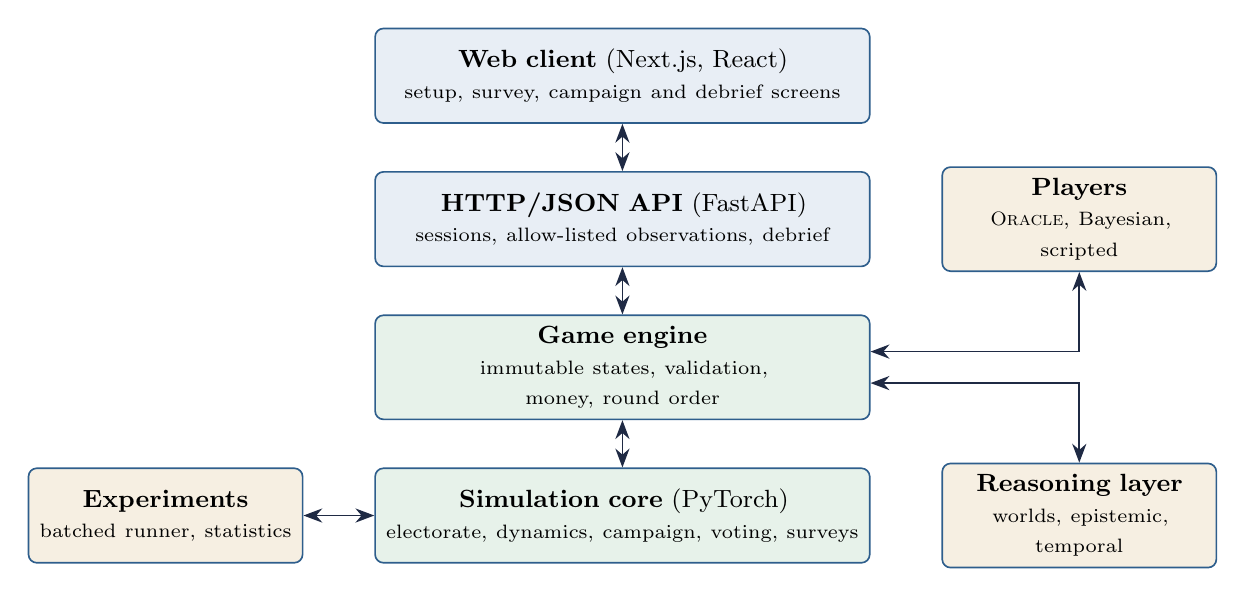
\begin{tikzpicture}[node distance=6mm and 9mm,
    every node/.append style={minimum height=12mm}]
  \node[box,text width=6.0cm] (web) {\textbf{Web client} (Next.js, React)\\
        {\scriptsize setup, survey, campaign and debrief screens}};
  \node[box,text width=6.0cm,below=of web] (api) {\textbf{HTTP/JSON API} (FastAPI)\\
        {\scriptsize sessions, allow-listed observations, debrief}};
  \node[boxg,text width=6.0cm,below=of api] (engine) {\textbf{Game engine}\\
        {\scriptsize immutable states, validation, money, round order}};
  \node[boxg,text width=6.0cm,below=of engine] (core) {\textbf{Simulation core} (PyTorch)\\
        {\scriptsize electorate, dynamics, campaign, voting, surveys}};
  \node[boxs,text width=3.2cm,right=of api] (players) {\textbf{Players}\\
        {\scriptsize \ORACLE, Bayesian, scripted}};
  \node[boxs,text width=3.2cm,right=of core] (logic) {\textbf{Reasoning layer}\\
        {\scriptsize worlds, epistemic, temporal}};
  \node[boxs,text width=3.2cm,left=of core] (exp) {\textbf{Experiments}\\
        {\scriptsize batched runner, statistics}};
  \draw[darr] (web) -- (api);
  \draw[darr] (api) -- (engine);
  \draw[darr] (engine) -- (core);
  \draw[darr] (players.south) |- ([yshift=2mm]engine.east);
  \draw[darr] (logic.north) |- ([yshift=-2mm]engine.east);
  \draw[darr] (exp) -- (core);
\end{tikzpicture}
\caption{Software architecture. Players and the reasoning layer see the game only through observations;
the experiment harness drives the simulation core directly for speed.}
\label{fig:arch}
\end{figure}

The code is organised as a Python package with one module per concern: \code{electorate},
\code{dynamics}, \code{voting}, \code{information}, \code{game}, \code{strategies}, \code{logic},
\code{analysis} (spectral and robustness tools) and \code{api}. The package has about 5,900 lines of
Python, the web client about 5,600 lines of TypeScript, and the experiment scripts about 13,000 lines.

\section{The game engine}

The engine is a set of pure functions over immutable game states. Applying an action returns a new state;
a rejected action returns the same state object with an error code (for example \code{INSUFFICIENT\_FUNDS}
or \code{INVALID\_PHASE}), so it cannot leave the game half-changed. Money is kept as exact decimals with
two places, so prices and treasuries never suffer rounding drift. The engine follows the round order of
\cref{fig:flow}: hires, one cascade hop, media, the social step with workers pinned, then new polls. The
election runs automatically after the last round.

\section{Reproducibility}

Every random draw comes from a named stream derived from a root seed: \code{regions}, \code{graph},
\code{preferences}, \code{attributes}, \code{zealots}, \code{workers}, \code{cascade}, \code{media},
\code{poll}, \code{election} and others. Streams are derived with a cryptographic hash, and per-round draws
use sub-seeds keyed by stream, round and player. Two consequences follow.
\begin{itemize}
  \item The same $N$ and seed produce a bit-identical electorate on any machine with the same PyTorch
        version, because the electorate is generated from CPU streams and then moved to the device. A
        player can share a seed and someone else can play the same world.
  \item A game can be replayed exactly from its seed and its list of actions. The reasoning layer relies on
        this to compute ground truth at earlier decision points.
\end{itemize}
Every experiment result also records its configuration, seeds, git revision, device, and library versions.

\section{GPU-first simulation}

All operations on voters are tensor operations; there are no Python loops over voters. The graph is stored
as an edge list plus a compressed sparse row view, so memory grows with the number of edges and an
$N\times N$ matrix is never formed. Every function in the simulation core accepts an optional leading batch
dimension, so the same code simulates one world or $B$ worlds at once.

Two uses of batching matter most.
\begin{itemize}
  \item \textbf{Inside players.} The Bayesian planner joins its eight sampled worlds into one disjoint graph
        and simulates all candidate plans in one call. The reasoning layer does the same for its outcome
        matrix.
  \item \textbf{In experiments.} A batched true-world runner plays $B$ complete games per call, each with
        its own world, manifesto, policy and random streams.
\end{itemize}
The single code path gives a strong correctness check. On the CPU, the batched runner is bit-identical to
the reference single-world simulator. On the GPU, it produces identical discrete outcomes (who is hired,
who converts, who wins), and its floating-point values agree to within $6\times10^{-8}$. Every experiment
ran a three-seed CPU-to-GPU parity check before its main run. Spectral quantities use SciPy's Lanczos
solver on the CPU for moderate $N$ and power iteration on the GPU for large $N$.

\section{Keeping hidden information hidden}

A game about knowledge is only meaningful if the player cannot peek. Observations, API responses, logs and
error messages are built by allow-listed serialisers that copy only public fields. A recursive leak test
walks every response and fails if it finds any voter-level preference, susceptibility, zealot flag, edge,
archetype or personality map, block probability or seed. Computer players receive a deep copy of their own
observation, so they cannot reach into the engine either. The post-game debrief is the only place where
hidden truth is shown, and only after the game is over.

\section{The web game}

Humans play through a browser. The engine is served by a FastAPI~\cite{fastapi} application with routes to
create a game, fetch the player's observation, ask a question, commit, allocate, skip a round, and fetch the
debrief and epistemic timeline. Each game has its own lock, and idle games are evicted when the server is
full. The client is a Next.js~\cite{nextjs} application with four screens.
\begin{enumerate}
  \item \textbf{Setup:} choose $N$, the number of rounds, the treasury and an optional seed.
  \item \textbf{Survey:} read the free statistics, ask questions, and design the manifesto with sliders and
        a doughnut chart.
  \item \textbf{Campaign:} a region map, a sample of the friendship network, a poll chart, the round's
        intelligence, an allocation panel and an optional round timer.
  \item \textbf{Results:} the outcome, a round-by-round look back, the hidden truth, the \ORACLE{} benchmark
        and the epistemic timeline.
\end{enumerate}
The network view draws a stratified sample of voters and the edges between them, since drawing ten thousand
nodes would be unreadable and would leak more structure than the census allows.

\section{Testing}

The repository contains over two hundred automated tests. They cover the statistical properties of the
generators (region floors, mean degree, Dirichlet means), invariants of the dynamics (preferences stay on
the simplex, workers and zealots never move), the cascade rules (one hop per round, the three-attempt
cap), exact money accounting, the phase machine and its error codes, the privacy leak test, the API
contract, the duality and other identities of the epistemic operators, and CPU-to-GPU agreement. Tests
that need a GPU skip automatically without one. The web client has unit tests and browser end-to-end tests.

\section{Experiment harness}

The experiments share a small library. Every arm of an experiment runs on the same seeds (a paired design),
and different experiment groups use disjoint blocks of seeds. Results are reported with 95\% Wilson
intervals for rates~\cite{wilson1927} and $t$-intervals for means; paired comparisons use the Wilcoxon
signed-rank test~\cite{wilcoxon1945} for differences in vote share and the exact McNemar
test~\cite{mcnemar1947} for wins, with the Holm--Bonferroni correction~\cite{holm1979} within each
experiment. Global sensitivity uses the Morris screening design~\cite{morris1991}.

Before each experiment ran, we wrote down what we expected it to show. Each experiment writes raw per-game
rows and a summary file, and every figure is redrawn only from those files. A checking script then reads
the written results and confirms that every number in the text appears, after rounding, in the data file it
cites.

\summarysection

The software is a layered Python package on top of PyTorch, with a game engine of pure functions over
immutable states, named random streams that make every game replayable, and a single tensor code path that
runs one world on a CPU or many on a GPU with verified parity. Allow-listed serialisers and leak tests keep
hidden information hidden. A FastAPI server and a Next.js client make the game playable in a browser, over
two hundred tests guard the rules, and a shared harness gives every experiment paired seeds, standard
statistics and machine-checked reporting. The next chapter reports what the experiments found.

%% =====================================================================
%%  Chapter 7: Experiments and results  (left empty on purpose)
%% =====================================================================
\chapter{Experiments and Results}\label{ch:results}

\overviewsection

\todo{To be written by the group.}

% Suggested structure (delete when filled in):
%   - Experimental setup and common protocol
%   - The goal: building consensus around the manifesto
%   - Mechanics against theory (consensus, cascade threshold, stubborn agents, submodularity)
%   - Strategy (tournament, plan search, manifesto)
%   - Information and knowledge (value of information, probing, verdict reliability, temporal properties)
%   - Design (balance, luck vs skill, misspecification, sensitivity)
%   - Scale and performance
%   - Prediction scorecard

\summarysection

\todo{To be written by the group.}

%% =====================================================================
%%  Chapter 8: Limitations and future work
%% =====================================================================
\chapter{Limitations and Future Work}\label{ch:limits}

\overviewsection

No model of an election is complete, and ours makes many simplifying choices on purpose. This chapter lists
the limitations that a reader should keep in mind when interpreting the results, and the directions we
would take the work next.

\section{Limitations of the model}

\begin{itemize}
  \item \textbf{A synthetic electorate.} Regions, archetypes, personalities and the network are drawn from
        distributions we chose. The parameters were tuned so that the game is playable and interesting,
        not fitted to any real electorate. Our conclusions are about this model, not about real elections.
  \item \textbf{One party.} There is no opponent. Voters either support the party or do not, so the game
        cannot show how two parties' manifestos would compete or converge.
  \item \textbf{Fixed manifesto.} The manifesto cannot be revised after it is committed, and there is no
        model of turnout beyond abstention.
  \item \textbf{A static network.} Friendships never change during a game, and edges are unweighted.
\end{itemize}

\section{Limitations of the method}

\begin{itemize}
  \item \textbf{References are heuristics.} The \ORACLE{} and the plan search are good players, not
        provably optimal ones. Any comparison against them measures distance to a strong heuristic, not to
        the true optimum.
  \item \textbf{Knowledge is sampled.} Epistemic and temporal verdicts are evaluated over finite samples
        of worlds, plans and futures, at a reduced number of voters. They are statements about the sample.
  \item \textbf{No human data.} All conclusions about play come from computer players. A planned human
        playtest was dropped for lack of time.
  \item \textbf{Shared hardware.} Experiments ran on shared GPUs, which affects measured timings but not
        results. CPU and GPU use different random streams, so their results agree statistically, not draw
        for draw, except where we checked parity.
\end{itemize}

\section{Future work}

\begin{itemize}
  \item \textbf{A human playtest.} Ask people to play the web game and compare their choices and outcomes
        with the computer players, and test whether the epistemic debrief helps them play better.
  \item \textbf{A second party.} Add an opponent and a multi-party voting rule, and study whether
        competing manifestos converge, as spatial voting theory predicts for two parties.
  \item \textbf{A language-model player.} The interface exists; implementing it would let us test how a
        general-purpose model reasons about a game with hidden information.
  \item \textbf{Exact or certified reasoning.} Replace sampled verdicts with bounds that hold for the whole
        information set, at least for small electorates.
  \item \textbf{Richer dynamics.} Bounded confidence, changing networks and weighted friendships would test
        how much our conclusions depend on the simple DeGroot rule.
\end{itemize}

\summarysection

The model is synthetic and has a single party, a fixed manifesto and a static network. Its reference
players are heuristics, its knowledge verdicts are sampled, and no human played the final version. The
most valuable next steps are a human playtest and a second party.

%% =====================================================================
%%  Chapter 9: Conclusion
%% =====================================================================
\chapter{Conclusion}\label{ch:conclusion}

\overviewsection

This chapter draws the report together: what we set out to do, what we built, and what we take away from
building it.

\section{What we did}

We set out to study an election campaign as a multi-agent system in which a party pushes on an electorate
that is already moving, and does so without seeing it. To make that concrete we built \emph{Dumbocracy}.
Its electorate combines DeGroot consensus, zealots and a stochastic block network. Its party workers are
stubborn agents that start an Independent Cascade. Its manifesto is a point on the simplex chosen by
projected gradient or ADMM. Its information model makes the player's knowledge an S5 information set that
can be sampled and reasoned about.

On top of the model we built players that see only what a human sees, including a Bayesian planner that
asks questions by information gain and plans by rollouts; a reasoning layer that tells a player, after the
game, what they knew and when the game was decided; a web interface; and a GPU-batched simulator that is
exact on the CPU and verified on the GPU. Together these turned the game into an instrument for testing
course theory with controlled, paired, pre-registered experiments, whose results are reported in
\cref{ch:results}.

\section{What we learned from building it}

Some lessons came from building the system rather than from the experiments.
\begin{itemize}
  \item \textbf{The anticipated electorate matters.} Optimising a manifesto against the voters as they are
        at the start is a mistake, because social averaging moves them before election day. Every good
        player optimises against where the electorate is going.
  \item \textbf{Mechanics and policy are coupled.} Because a voter's conversion chance depends on how much
        they already like the manifesto, the choice of manifesto changes how far workers' influence
        spreads. The ``policy'' and ``network'' halves of the game cannot be designed separately.
  \item \textbf{Knowledge needs care to compute honestly.} Keeping what the player knew separate from what
        was true required explicit reconstruction of earlier observations, a strict privacy boundary and
        exact replay.
  \item \textbf{One code path pays off.} Writing the simulator once, with a batch dimension, gave us both a
        reference implementation and a fast one, and made parity a test rather than a hope.
\end{itemize}

\summarysection

We built a game that brings consensus, contagion, optimisation, planning and logic together around one
model, and used it to study campaigning on a social network under uncertainty. The code is public at
\repo, and every result can be reproduced from it.

%% =====================================================================
%%  References
%% =====================================================================
\clearpage
\addcontentsline{toc}{chapter}{References}
\bibliographystyle{plainnat}
\bibliography{references}

%% =====================================================================
%%  Appendices
%% =====================================================================
\appendix

\chapter{Notation and Default Parameters}\label{app:notation}

\section*{Notation}

\begin{table}[h]
\centering
\caption{Notation used in the report.}
\label{tab:notation}
\small
\begin{tabularx}{\linewidth}{@{}lX@{}}
\toprule
Symbol & Meaning \\
\midrule
$N$, $T$            & number of voters; number of campaign rounds \\
$r$, $n_r$          & region index (North, South, East, West); number of voters in region $r$ \\
$\simplex$          & the probability simplex of budget splits over five sectors \\
$v_i \in \simplex$  & voter $i$'s preferred budget split (hidden) \\
$b \in \simplex$    & the player's manifesto \\
$\sigma$, $\tau$    & hidden maps from regions to archetypes and to personalities \\
$\theta = (\sigma,\tau)$ & hidden type of a world (8640 possibilities) \\
$\alpha_i,\beta_i,\gamma_i$ & susceptibility to friends, media and canvassing \\
$S_i$               & agreement with the manifesto, $1 - \tfrac12\lVert v_i - b\rVert_1$ \\
$P_i$               & probability that voter $i$ votes for the party \\
$E$                 & expected vote share, the mean of $P_i$ \\
$A$, $D$, $L$       & adjacency, degree and Laplacian matrices of the friendship graph \\
$W_t$, $\Pi_t$      & sampled consistent worlds and plan set at decision point $t$ \\
$\Kop$, $\Mop$      & knowledge and possibility operators \\
\bottomrule
\end{tabularx}
\end{table}

\section*{Default parameters}

\begin{table}[h]
\centering
\caption{Default parameters of the v3 game.}
\label{tab:params}
\small
\begin{tabularx}{\linewidth}{@{}Xll@{}}
\toprule
Parameter & Symbol & Default \\
\midrule
Number of voters                          & $N$            & $10^4$ (allowed $10^3$ to $10^6$) \\
Campaign rounds                           & $T$            & 5 (web game 3 to 5) \\
Treasury                                  & --             & \coins{500} (allowed 500 to 1000) \\
Minimum region share                      & --             & 15\% \\
Mean degree                               & $\bar k$       & 30 \\
Within-region link weight                 & $p_r$          & $U[0.5, 0.9]$ \\
Between-region link weight                & $p_{rs}$       & $U[0.01, 0.2]$ \\
Dirichlet concentration                   & $\kappa$       & 60 \\
Zealot fraction                           & $\zeta$        & 0.05 \\
Social step                               & $\omega$       & 0.15 \\
Worker price                              & --             & \coins{20}, paid once \\
Worker minimum degree; attempt cap        & --             & 3; 3 per voter per game \\
Media base price                          & $m_0$          & \coins{50} per quarter-sized region \\
Media reach; strength; decay              & $p_m,\eta_0,\lambda$ & 0.6; 0.25; 0.5 \\
Vote slope; threshold                     & $\beta_v$, $z$ & 20; 0.825 \\
Survey price; sample fraction             & --             & \coins{10}; 10\% of the region \\
Free poll size                            & --             & 400 voters \\
\bottomrule
\end{tabularx}
\end{table}

\chapter{Reproducing the Work}\label{app:repro}

All code is in the public repository \repo. The commands below assume a Python 3.11 or newer environment
and, for the web game, Node.js 22.

\paragraph{Install and test.}
\begin{verbatim}
pip install -e '.[web,analysis,test]'
python -m pytest -q          # GPU tests skip without CUDA
\end{verbatim}

\paragraph{Play the game.}
\begin{verbatim}
scripts/run_game.sh          # engine on :61008, web client on :61007
\end{verbatim}

\paragraph{Run an experiment and redraw the figures.}
Each experiment is one script in the \code{experiments} folder, for example \code{x6\_tournament.py} for
the strategy tournament. The exact command line of every run is stored in its result file, in the field
\code{provenance.command}.
\begin{verbatim}
python experiments/x6_tournament.py --device cuda:0
python experiments/plot_v3.py
python experiments/x_report_check.py
\end{verbatim}
The last command checks every number in the results write-up against the data file it cites.

\end{document}
